\chapter{Development follow up}
In this chapter, we will follow development of each milestone. For each one, first, we will describe the issues involved. Then, we will describe the design decisions made, and finally, we will discuss interesting lessons and problems we have encountered in that iteration.

The Github repository used for the development of this project can be found at \href{https://github.com/salvacorts/TFG-Parasitic-Metaheuristics}{github.com/salvacorts/TFG-Parasitic-Metaheuristics}.

\section{Demo Problem}
This milestone contained the following user story:

\subsubsection*{\href{https://github.com/salvacorts/TFG-Parasitic-Metaheuristics/issues/20}{Issue \#20}: As an Administrator, I want to run a demo problem so that I can test the platform} 

Fist of all, we need a problem that can perform well in the platform. This problem will be used to test the platform as we develop it further.

We chose a multilayer perceptron (MLP) trained with the \textit{Glass} and \textit{Cancer1a} datasets from \textit{proben1} benchmark \ref{proben1}; a set of benchmarks for neural network training algorithms.

The \textit{Glass} dataset is made of 214 samples of glass where each one contains the percent content of 8 different chemical elements, its refractive index, and the type of glass (class attribute). A model that can predict the kind of glass from new samples, can be useful in criminal forensics.

\textit{Cancer1a} is made of 699 samples of breast cancer. Each one contains a sample identification number, 9 attributes about the cell that the sample measures, and the class of cancerous cell: either benign or malignant.

There are two main reasons to have chosen a multilayer perceptron to develop and demo the platform. On the one hand, its fitness function takes more time than the average latency of communication between nodes in the platform. On the other hand, we have previous experience \ref{gprop} with this problem and we are familiar with some useful genetic operators we can apply.

The genetic operators of the genetic algorithm we will use to optimize the neural network are the same ones proposed by P. A. Castillo et al in G-Prop \cite{gprop}:

\begin{itemize}
	\item \textbf{Selection:} Roulette tournament where two chromosomes are randomly selected from the population to cross.
	
	\item \textbf{Evaluation:} Train a copy of the chromosome with the training dataset without Backpropagation. The fitness of the chromosome that will be returned by this operator will be the classification error obtained by predicting new samples from the validation dataset with the trained copy of the chromosome.
	$$ Error = 1 - \frac{TP + TN}{TP + TN + FP + FN}  $$
	
	Where $TP = $ True Positives, $TN = $ True Negatives, $FP = $ False Positives, and $FN = $ False Negatives.
	
	\item \textbf{Mutation:} First, modify the learning rate of the network by adding a random number uniformly distributed in the range [-0.05, 0.05]. Then, with certain probability, for each neuron in each hidden layer (in our case there is just one hidden layer), add a random number in the range [-0.1, 0.1] following uniform distribution to all its weights.
	
	\item \textbf{Crossover:} Apply a multi-point crossover between two chormosomes where the neurons of both parents will be mixed resulting in two new offspring that will contain neurons from both parents. The learning rates of the two parents are swapped as well.
	
	\item \textbf{Add Neuron:} Add a new randomly initialized neuron to the hidden layer that will be connected with the neurons in the following and previous layer. This operator performs incremental learning and attempts to address the problem of estimating the number of neurons to use in the hidden layer.
	
	\item \textbf{Eliminate Neuron:} Remove a randomly selected neuron from the hidden layer performing decremental learning. This operators aims to reduce the risks of over-fitting due to having too many neurons in the hidden layer.
	
	\item \textbf{Substitute Neuron:} Replace a random neuron from the hidden layer with a new one randomly initialized.
	
	\item \textbf{Train:} This operator performs a local search by training the multi-layer perceptron represented in the chromosome with Backpropagation \cite{backpropagation} for a given number of epochs.
\end{itemize}

We have developed our evolutionary algorithm using the \textit{Go} language \cite{go}. Go, or Golang, is a is a statically typed and compiled open-source programming language that features a C-like syntax but that comes with garbage collection and built-in easy support for concurrent and distributed programming thanks to its \textit{goroutines} \cite{channels} and \textit{channels} \cite{channels}.

There are two main pre-existing libraries that we will use:

\begin{itemize}
	\item \textbf{Go Perceptron:} A single and multilayered perceptron classifier trained with Backpropagation \cite{go-perceptron-go}.
	\item \textbf{eaopt:} An evolutionary optimization library that supports various evolutionary optimization algorithms such as genetic algorithms, particle swarm, and differential evolution among others. It also provides different genetic algorithm models, selection, mutation and crossover operators out of the box \cite{eaopt}.
\end{itemize}

\subsubsection*{Implementation}
As deliverable prototype for the end of this milestone, we wanted to have the same solution running on both native and browser environments. Typically we would have had to write the same code twice; in Go for native and in Java Script for the browser, but thanks to WebAssembly, we could share the same code base between both native and browsers with just minor changes.

The \textit{Go perceptron} library fitted our necessities well so we didn't need to modify it internally at the very first moment. On the other hand, we had to modify \textit{eopt} so we could execute other genetic operators over the population apart from the mutation, evaluation and crossover operators.

In order to use eaopt, first the developer needs to configure the number of generations, the population size and the genetic model to use in the genetic algorithm. The model defines how the algorithm evolves the population with the selection, mutation and crossover operators; in our particular case, we decided to use a generational model.

\begin{lstlisting}[
caption={eaopt's Genome interface},
label={lst:ExtraOperator}, captionpos=b]
type Genome interface {
	Evaluate() (float64, error)
	Mutate(rng *rand.Rand)
	Crossover(genome Genome, rng *rand.Rand)
	Clone() Genome
}
\end{lstlisting}

Since the implementation of these models does not contemplate additional genetic operators apart from those defined in the \textit{Genome} interface from \textit{eaopt}, we had to add an additional member to the generational model class containing an array of extra genetic operators (Listing \ref{lst:ExtraOperator}) that are used after applying mutation and crossover over a given chromosome as seen in Listing \ref{lst:opapp}.

\begin{lstlisting}[
caption={Definition of an extra genetic operator as a struct with a float representing the probability op application, and a function that takes genome and returns a modified one.},
label={lst:ExtraOperator},
captionpos=b]
type ExtraOperator struct {
	Operator    func(Genome, *rand.Rand) Genome
	Probability float64
}
\end{lstlisting}

\begin{lstlisting}[
caption={Application of extra operators after mutating.},
label={lst:opapp},
captionpos=b]
// Apply mutation to the offsprings
if mod.MutRate > 0 {
	offsprings.Mutate(mod.MutRate, pop.RNG)
}

for i := range offsprings {
	for _, operator := range mod.ExtraOperators {
		if operator.Probability > 0 {
			if pop.RNG.Float64() < operator.Probability {
				offsprings[i].ApplyExtraOperator(operator, pop.RNG)
			}
		}
	}
}
\end{lstlisting} 

As soon as the the genetic operators were implemented and tested, we proceeded to fully execute the genetic algorithm.
In order to get some insights about the state of the population during the execution of the genetic algorithm, we logged the fitness and the number of neurons of the best chromosome, and the average fitness of the population after each generation. In Figure \ref{native}

\begin{figure}[h!]
		\centering
    	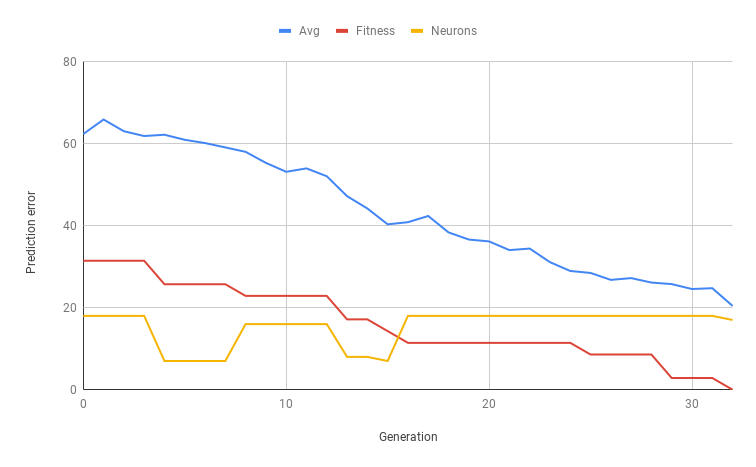
\includegraphics[width=\linewidth]{assets/images/milestone1-native-chart.png}
    	\caption{Evolution of the fitness as error predicting the validation dataset and the neural network size}
    	\label{fig:native}
\end{figure} 

We noticed that the execution of the algorithm was taking too long so we used a profiler in order to study which areas of the code were taking most time. It ended up being the \textit{Go perceptron} logs generator. we disabled these logs and the execution time was dramatically increased from more than 30 minutes to around 2 minutes.

Once we were happy about the results, we started to build a simple web interface as a proof of concept for the execution of the algorithm compiled into WebAssembly.


Talk about the results and time in Wasm

